\documentclass{book}
\usepackage[utf8]{inputenc}
\usepackage[spanish]{babel}
\usepackage{graphicx}
\usepackage{graphicx,subfig}
\usepackage{mathptmx}
\usepackage{multicol}
\usepackage{color}
\usepackage{listings}
\usepackage[usenames,dvipsnames,svgnames,table]{xcolor}

\addto\captionsspanish{\renewcommand{\contentsname}{CONTENIDO}}

\begin{document}
	\thispagestyle{empty}
	\frontmatter
	\begin{minipage}{.3\textwidth}
	\begin{flushleft}
		\begin{center}
			{
\includegraphics[scale=.35]{Assets/images/escudo_unam.png}}
		\end{center}
		\vspace{10pt}
		\begin{center}{
				\rule{.5pt}{.6\textheight}
				\hspace{7pt}
				\rule{2pt}{.6\textheight}
				\hspace{7pt}
				\rule{.5pt}{.6\textheight}
			}
		\end{center}
		\begin{center}{
\includegraphics[scale=1]{Assets/images/escudo_fi.jpg}}\end{center}
	\end{flushleft}
	\end{minipage}
	\begin{minipage}{.7\textwidth}
		\begin{flushright}
				\begin{center}
				\begin{center}
					\LARGE{U}\large{NIVERSIDAD} \LARGE{N}\large{ACIONAL} 
					\LARGE{A}\large{UTÓNOMA} \\[10pt]
					\large{DE} 
					\LARGE{M}\large{ÉXICO} 
				\end{center}
				\rule{\textwidth}{2pt}
				\\
				\hrulefill\\[1cm]
				
				\LARGE{F}\large{ACULTAD DE } \LARGE{I}\large{NGENIERÍA}\\[2cm]
				
				\large{Diseño e implementación de un entorno computacional para la ayuda en la síntesis de sonidos musicales}\\[1.5cm]
				
				\huge{T E S I S }\\[1.5cm]
				
				\large{QUE PARA OBTENER EL TÍTULO DE:}\\[1cm]
				
				\large{INGENIERO EN COMPUTACIÓN}\\[1cm]
				
				\large{PRESENTA}
				
				\large{Joaquín Gustavo Espino de Horta}\\[1cm]
				
				\large{DIRECTOR DE TESIS}
				
				\large{Dr. Rogelio Alcántara Silva}\\[1cm]
				
				\large{Ciudad Universitaria, Cd. Mx., Agosto 2024}
				
			\end{center}
		\end{flushright}
	\end{minipage}
	
	\section*{Agradecimientos}
	Tras muchos años en pie de lucha contra las adversidades internas y externas, finalmente puedo tomarme un respiro para mirar atrás, me sorprende la cantidad exacta del tiempo tomado hasta este punto, tan corta para ser toda mi historia y mucha para ignorar su significante legado. Desde las tareas más simples hasta aquellos desafíos aún en este día de aspecto desafiante. Solo puedo dar un suspiro como agradecimiento en esta posición.\par 
	
	Duele mucho el ya no tener un propósito por el cual diste la vida, finalmente tienes la libertad y ahora sientes frío donde antes estaban tus grilletes, es donde puedes recuperar tu humanidad perdida, el gran precio a pagar por más horas extra en tus estudios, recordar aquellos nombres de quienes estuvieron en un momento, voltear y llamarlos amigos, familia o amada. Si bien no es un final donde no queda nada por hacer, es donde finalmente podemos construir el sueño, con los escombros y herramientas adquiridas a lo largo de tantas vivencias en nuestra particular situación.\par 
	
	Mi deber es levantarme y seguir sin bajar mi mirada en los objetivos, avanzo, camino, troto y corro alegre cual niño en su incompresible alegría. \emph{Después de todo, sigues siendo tú.} Aquel niño repleto de sueños, historias e ideas por contar y compartir a su alrededor. No guardo odio o rencor, sino buenos recuerdos como Heródoto y experiencias para el futuro como Tucídides, así puedo avanzar y disfrutar de la vida a cual me tocó estar.\par 
	
	Para toda mi familia, siempre supe esperaban mucho de mi y espero así esto sea de su consideración, cada disgusto y sacrificio sea compensado con estas acciones. Mamá y Papá, espero haber sido un buen hijo y haberme ganado mi libertad. Tíos y Primos, gracias por su fé y enseñanzas. A los que ya no están, lamento haberme tardado tanto, ahora podré honrarlos de la mejor manera.\par
	
	Para todos mis amigos y conocidos, gracias por cada charla, consejo y diversión. Los considero mis hermanos, Fernando, Armando, Daniel, Victor, Juan Bedolla, Erick, Gabriel, Humberto, como todos a quienes he conocido, a mis mejores amigas por sanar mis heridas, Maricela, Dianita, Violeta, Mitzi... por su hombro cuando necesitaba llorar.\par
	
	Para mi querida Danna, aún cuando nos falta mucho por vivir y superar, confío en aquello lo cual no puedo controlar para un mejor futuro. Y en aquello de lo cual puedo controlar y mi DETERMINACIÓN siempre será a un destino juntos.\par
	
	Buenas noches y la armonía esté con todos ustedes.\par
	
	\begin{flushright}\emph{- Joaquín Gustavo Espino de Horta}\\ \emph{"JoGEHrt"}\end{flushright}
	
	\pagebreak\section*{RESUMEN}
	Con el fin de facilitar la producción de audio con enfoques al público general, de maneja semejante al impacto de herramientas computacionales, se postula la creación de modelos reproducibles y económicos en procesamiento como almacenamiento en memoria sobre un nuevo formato para el desarrollo, en un ambiente computacional integral sencillo de entender y manejar. De esta manera, se espera ofrecer una nueva alternativa a la composición musical que exija menos recursos externos y computaciones en sus formas de almacenar y replicar.
	\section*{OBJETIVOS}
	\begin{itemize}
		\item Construcción de una interfaz de usuario para la ayuda visual y auditiva en la composición y síntesis de sonidos.
		\item Implementación del los modelos generados en otros ambientes de software.
	\end{itemize}
	\tableofcontents\pagebreak\setcounter{page}{0}
	
	\markboth{Introducción}{Introducción}
	\section*{INTRODUCCIÓN}\addcontentsline{toc}{section}{Introducción}
	La interpretación de información en nuestros medios digitales, nos ha permitido producir y almacenar de forma eficiente y a un nivel mínimo de personal, siendo un ejemplo, solo se requiere un procesador de texto instalado en un equipo para poder construir artículos, publicaciones y gran diversidad de documentos formales, informales, con propósitos de cualquier índole o ámbito del cual se requiera constancia y permanencia para su divulgación.\par
	Todo lo anterior mencionado, gracias a los productos de software comercial disponibles, tanto en la producción de su contenido objetivo, como sus respectivos entornos de trabajo integrales para su construcción en un proceso más individual ó en un ámbito industrial, como su manutención.\par
	Enlazando ambos conceptos, propongo aplicarlos a un ámbito artístico muy computable gracias a su amplio análisis matemático-lógico. Hablo de la música, disciplina artística de la armonía del sonido, su composición e interpretación, creada a partir de la refinación en las ondas sonoras a gusto y agrado del contexto social.\par 
	Perfectamente replanteadas en modelos trigonométricos, así como la captura de su información con el uso de archivos especializados en su fidelidad, compresión y réplica.
	Visto de otra manera, la información contenida en un archivo de audio, da las instrucciones y valores de comportamiento para un dispositivo de salida sonoro.\par 
	Sin importar el origen de esta información, por una captura directa, una copia de otro archivo, mezclado y renderizado por un programa de edición o incluso de la muy improbable casualidad. Solo se requiere de un método adecuado de producción.\par
	Si el desafío reside en la fuente de origen, entonces se propone \emph{La construcción de una interfaz de usuario para la ayuda visual y auditiva en la composición y síntesis de sonidos.}
	De acuerdo con el teorema de Fourier, referente a la descomposición en señales de onda para cualquier señal periódica. Será la fundamental relación de nuestra propuesta. Pues con la ayuda visual y auditiva en comparar por el oído y vista un modelo generado con respecto a una muestra recolectada, la réplica fidedigna a criterio de la escucha del público objetivo de producto final.\par 
	Esta idea tiene su génesis en el proyecto de sintetizador creado por el usuario \emph{Javidx9/OneLoneCoder}, una plantilla hecha en lenguaje C++ que se puede encontrar en el siguiente repositorio: \color{blue}https://github.com/OneLoneCoder/synth.git \color{black}\\En este se expresan mediante objetos virtuales construidos sobre código duro(Hardcode) funciones trigonométricas de oscilador hechas para la réplica de notas musicales y como en variaciones de amplitud y frecuencia pueden emular instrumentos simplificados.\par
	Así se espera, construir una forma de replicar el audio en tiempo de ejecución, pudiendo aplicar un nuevo panorama de beneficios y propuestas de solución a los ámbitos para la producción de contenido, especialmente aquellas interactivas.\par
	\pagebreak
	\begin{minipage}{.7\textwidth}
		\begin{flushleft}
			\vspace{10pt}
			\begin{center}
				\Large{VISIÓN}
				\hrulefill\\[1.5cm]
			\end{center}
		\end{flushleft}
	\end{minipage}\par
	La siguiente imagen muestra una representación simplificada sobre la propuesta de solución al completo, donde se tiene planeadas todas sus funcionalidades y operaciones al menos de cara a un lanzamiento hacia el público interesado, más no uno comercial.\par
	
	Están contempladas 5 grandes aspectos para el desarrollo de una aplicación integral, aunque se aclara desde este punto, solo se centrará en un módulo, el más significativo en cuanto una nueva propuesta se refiere. Siendo el módulo de \emph{Tuner} (afinador).
	\begin{figure}[h]
		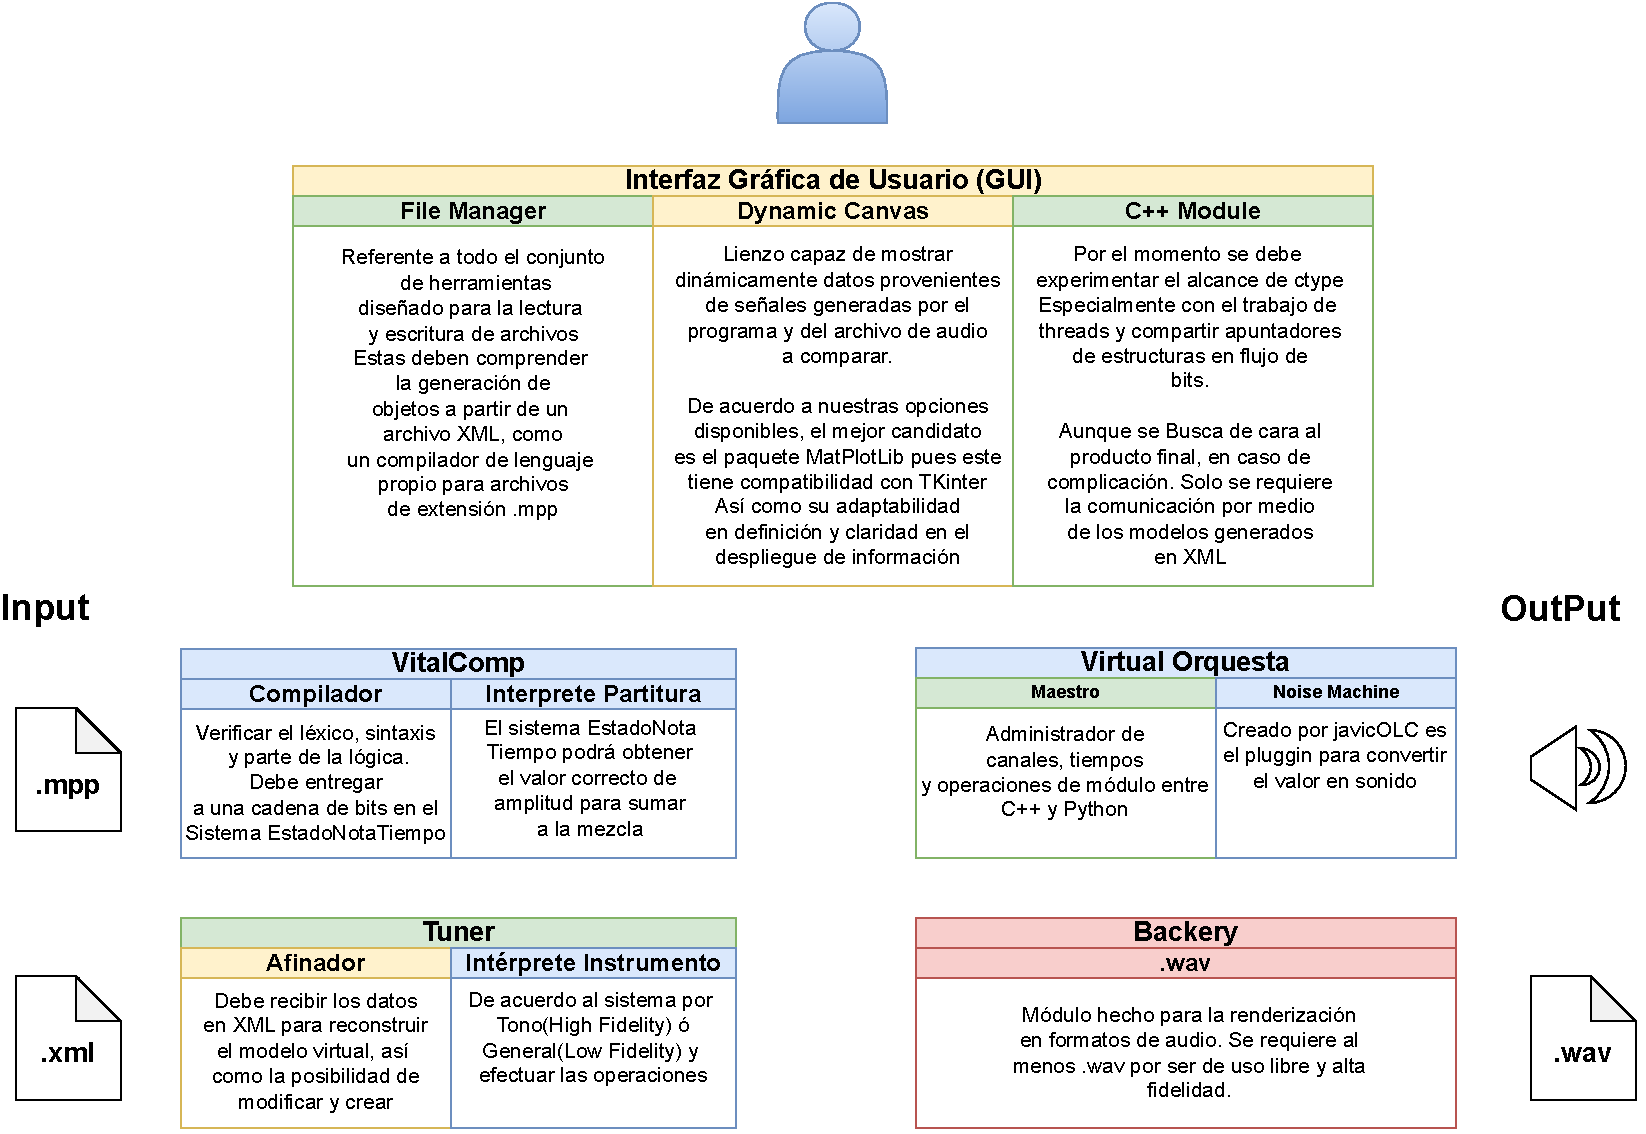
\includegraphics[width=1.25\linewidth]{Assets/images/musiC++_Diagram}
		\caption{ Diagrama General del Proyecto Completo}
	\end{figure} 
	
	\pagebreak
	\begin{minipage}{.7\textwidth}
		\begin{flushleft}
			\vspace{10pt}
			\begin{center}
				\Large{MÓDULOS}
				\hrulefill\\[1.5cm]
			\end{center}
		\end{flushleft}
	\end{minipage}\par
	Profundizando en los módulos mostrados anteriormente:\par
	{\Large Interfaz Gráfica de Usuario (GUI)}\par
	El enfoque comercial del proyecto, exige que este contenga por lo menos una visualización cercana a los estándares en herramientas de software, si bien, el público general cambia su tendencia en cuanto conocimientos informáticos básicos, sería un error cerrarnos de cara a una presentación como la manipulación para una terminal de consola. Se ha experimentado construir una GUI con el lenguaje \emph{C++}, sin embargo no pudo encontrarse una biblioteca adecuada, mucho menos un resultado satisfactorio para delegar todo el proyecto a un único lenguaje de programación, por lo tanto, se trabajará con Python en el \emph{FrontEnd}, es decir, todo contacto con el usuario final.\par
	{\large File Manager}\par
	Ya que nuestro propósito es la generación de archivos cuya información pueda interpretarse por un estándar orientado a audio, así como la preservación del trabajo en un lenguaje de programación, es imperativo usar varios sistemas de lectura y escritura de archivos en ambos lenguajes a utilizar, siendo \emph{Python} y \emph{C++}, estos contienen una biblioteca en sus paquetes fundamentales, siendo la función \emph{open} y \emph{fstream} respectivamente. Por otra parte, se necesitará de una biblioteca especializada en convertir la información de un texto etiquetado como lo es el formato XML. No solo es un estándar que permite escalar las funciones del proyecto a futuro con otros productos de software, sino que al ser un formato simple y en cierto punto, indicativo para ser editado manualmente.\par
	{\large Dynamic Canvas}\par
	Si bien, esta parte podría únicamente ser útil en lo que respecta la construcción del módulo afinador. Puede utilizarse en tiempo real la representación gráfica de la información generada, desde los armónicos que participan en la mezcla del sonido, una visión más amigable de cara al usuario de los eventos programados, entre otras cosas. Ya que esto está ligado a la GUI así como el afinador, su desarrollo sería exclusivamente en Python, optando por la opción que ofrece el paquete de MatPlotLib por su compatibilidad con TKinter\par
	{\large C/C++ Module}\par
	Debido a las características por implementar, es conveniente dejar a Python como aquel que tenga el ejecutable inicial, así como ser el eje de las herramientas que conlleve el proyecto. Este ofrece una opción denominada como \emph{ctype} el cual permite convocar código en \emph{C/C++} colocando y devolviendo datos primitivos, aún no se ha experimentado del todo, pues se requiere de la certeza y técnicas en cuanto el envío de apuntadores para arreglos de datos, estructuras específicas así como su correcto funcionamiento con múltiples hilos de ejecución.
	
	\pagebreak{\Large VitalComp}\par
	Este módulo comprende el lenguaje de programación propuesto para la codificación de melodías en cuanto Tonos y Tiempos se refiere, así como su manejo en melodías. El nombre es en conmemoración a un profesional en la música, conocido personal, \emph{Vitalis Elrich} a quien se le había consultado la idea inicial y gracias al estudio de necesidades y herramientas actuales en el mercado, se sugirió la propuesta sobre un lenguaje de programación.\par
	{\large Compilador}\par
	El compilador estará compuesto por 2 fases (independientes al análisis léxico, semántico y lógico), pues se plantean 2 paradigmas distintos en un mismo formato, pues por un lado tendríamos las necesidades logísticas en cuanto a la sincronización, designación de tiempos, incluso la posibilidad de implementar una aritmética y lógica primordiales con el fin de hacer compatible con otros códigos.
	Para su construcción, se emplearán los recursos de \emph{Flex} y \emph{Bison} para las primeras etapas, donde se obtendrá una cadena atómica verificada en la que se interpretarán parcialmente los comandos y símbolos para la adecuación del ambiente al momento de recibir la segunda fase, esta consistirá en reconocer elementos melódicos como el nombre de las notas(pueden ser católicas o protestantes), comandos referentes a acordes específicos, así como la duración, varianza en semitonos entre otras características que pueda contener una partitura y ser representada en comandas. Para este último conviene manejarse en un detector de símbolos para la reducción atómica y el complemento en una cadena de Bytes, por medio de un estado universal que tenga tiempos por defecto así como los propios modos... Así estamos solucionando el uso dinámico pues al ejecutarse condicionalmente, la computadora podrá re-compilar las partes móviles\par
	{\large Intérprete}\par
	Ajustando el proyecto original del usuario \emph{Javidx9/OneLoneCoder}, se parte de modificar la estructura \emph{sequencer}, cuya función principal es la generación automática de información en tiempos y notas para que sean añadidas en el mecanismo principal. Si bien, su versión está limitada a una sola característica, pues fue diseñada como un efecto cíclico de batería. Rescatando el concepto abstracto del secuenciador, es posible modificar a un sistema de interpretación por cadenas de Bytes, inspirado en el \emph{pipeline de renderizado} usado en procesos gráficos de \emph{OpenGL}. Esta consiste en la toma de 3 Bytes con información de tipo Estado, Timbre y Duración, por cada Tempo en secuencia de melodía, es decir, que clase de sonidos, su tiempo en reproducción y el estado técnico para poder formar acordes, silencios o incluso solicitar una interpretación especial(fuera de mayores ó bemoles) en relación con otras notas. Cabe abordar una sugerencia en cuanto la optimización del caso estático, pues si la máquina no contiene ninguna variación, porque de ser el propósito: generar un archivo en memoria de almacenamiento, entonces, no debería compartir el mismo mecanismo en tiempo real, ahorrando recursos de presentación y otorgando una mayor eficiencia de uso.\par
	
	\pagebreak{\Large Virtual Orquesta}\par
	Este es un módulo enfocado al procesamiento central de la información, pues estará diseñado para invocar la interpretación de las instrucciones y ajustes dados por el usuario, administración de los múltiples hilos dedicados, pausa, reinicio, incluso a la captura en tiempo real de notas generadas por el usuario mediante una entrada estándar así como la posibilidad de escalar a un instrumento especializado.\par
	{\large MasterChord}\par
	Siendo esta parte administrativa, deberá cumplir con una facilidad de funciones que puedan ser citadas como servicios desde la GUI así como la respuesta de información siendo instrumentos, posición de notas, tiempo real o cualquier información correspondiente a una visualización con propósitos artísticos o técnicos. Si bien las funciones gráficas son prescindibles, se deja abierta la posibilidad de escalar al producto final.\par
	{\large NoiseMachine}\par
	Esta es una cabecera hecha por \emph{Javidx9/OneLoneCoder} que nos permite la comunicación con el hardware hecho para la reproducción de audio mediante la solicitud del tiempo en valor de la amplitud otorgado por una función asignada. Esta pieza limita el proyecto a plataformas con sistema operativo Windows 7 en adelante, con compatibilidad para arquitectura de x32 bits.\par
	{\large Backery}\par
	Recordando los propósitos iniciales, es evidente la necesidad de respaldar los archivos en memoria de almacenamiento, por lo tanto necesitamos de alguna forma, guardar la información en un estándar para la reproducción de audio.\par
	
	\pagebreak{\Large Tuner}\par
	{\large Generador de Señales}\par
	{\large Virtual Instrument}\par
	
	\pagebreak Para la realización de estos se ha tomado como base un proyecto para emulación de instrumentos del talentoso ingeniero inglés conocido en sus redes sociales electrónicas como \emph{Javidx9}. Su proyecto \emph{olcNoiseMaker} sienta los principios para estos requisitos:\vspace{2mm}
	
	\textbf{Maestro del Audio}
	{\tiny \lstinputlisting[language=c, firstline=381, lastline=403]{Assets/code/main4.cpp}}
	\textbf{Plantilla de Instrumento}
	{\tiny\lstinputlisting[language=c, firstline=183, lastline=209]{Assets/code/main4.cpp}\pagebreak}
	\textbf{Acceso a Hardware}
	{\tiny\lstinputlisting[language=c, firstline=183, lastline=252]{Assets/code/olcNoiseMaker.h}\pagebreak}
	\pagebreak\section*{Resultados Esperados}
	El producto en su finalidad debe ser capaz de:
	\begin{itemize}
		\item Bajo en consumo de recursos computacionales
		\item Utilizable en muchos entornos de programación
		\item Facilidad en su comprensión para el usuario
		\item Simulación de instrumentos musicales diversos
		\item Diseño escalable al número de funciones y modos
		\item Grabar los formatos más utilizados en la actualidad
	\end{itemize}
	Respecto a la funcionalidad, esta deberá estar accionada desde una entrada estándar en cadena de texto. Dando como una salida la reproducción del sonido esperado, como su posibilidad de almacenarse en los formatos objetivo.\vspace{2mm}
	
	De esta manera, se espera un uso por parte de usuarios desde aplicaciones sofisticadas con una interfaz gráfica de usuario agradable a la vista, como las opciones comerciales presentadas hasta la implementación en lenguaje de alto nivel. Se tiene como panorama el paradigma de interpretación y lectura secuencial gracias a sus propiedades fundamentales arraigadas en las características de computadoras comerciales accionadas por sistemas Linux ó Windows, así como su vista hacia Android.\vspace{2mm}
	
\end{document}

